% !TeX root = ../main.tex
% Add the above to each chapter to make compiling the PDF easier in some editors.

\chapter{Implementation}\label{chapter:implementation}

The following sections describe the implementation and explain the design decisions we made during development. 

\section{Technology Stack}

As our mobile platform, we have to decide between iOS and Android. While iOS has a more up-to-date operating system with 70\% of all of their mobile phones running iOS 13 and 23\% running iOS 12, Android has a much bigger market share with around 74\% compared to Apple's 25\%. 
% Todo: \cite[https://www.statista.com/statistics/272698/global-market-share-held-by-mobile-operating-systems-since-2009/]
% Todo: \cite[https://gs.statcounter.com/os-market-share/mobile/worldwide]

In terms of available development kits and libraries, both platforms provide plenty of choices. In the end, we choose Android, mainly because of their ease of deployment on devices for test scenarios. As for programming language, we opt for Kotlin instead of Java because of their intuitive syntax and compact and more readable codebase.

On the server-side of development, we select Node.js using Typescript combined with MongoDB's cloud storage solution, Atlas. Node.js provides a lot of flexibility with its vast ecosystem of third-party packages, and MongoDB, as a NoSQL database, easily stores and combines any type of data, allowing quick changes in the data model.
% Todo: \cite[https://nodejs.org/en/]
% Todo: \cite[https://www.mongodb.com/cloud/atlas]

Our aggregation results can be fetched over the REST API or viewed directly in the MongoDB Atlas interface, given access privileges.

\section{REST API}
\label{sec:api}
We use a REST API based on the JSON data exchange format, and the endpoints are shown in the Table \ref{tab:rest}.

\begin{table}[htbp]
\centering
  \begin{tabularx}{0.92\textwidth}{|l|X|}                                                                             \hline
		\multicolumn{1}{|c|}{\textbf{HTTP call}} & \multicolumn{1}{c|}{\textbf{Description}} \\ [0.5ex] 
		\hline
		POST /crowd HTTP/1.1 & Creates a new user and returns a password \\
		\hline
		POST /crowd/ping HTTP/1.1 & Updates the latest timestamp to current time \\
		\hline
		POST /aggregationRequest HTTP/1.1 & Initiates a aggregation request and forwards them to the device groups \\ 
		\hline
		POST /aggregationsteps HTTP/1.1 & Sends the intermediate step results of a group to the server for further processing  \\ 
		\hline
		POST /aggregationactivity HTTP/1.1 & Sends the intermediate activities results of a group to the server for further processing  \\ 
		\hline
		POST /aggregationlocation HTTP/1.1 & Sends the intermediate loaction results of a group to the server for further processing  \\ 
		\hline
		POST /aggregationpresence HTTP/1.1 & Sends the intermediate presence results of a group to the server for further processing  \\ 
		\hline
		GET /aggregationResult HTTP/1.1 & Retrieves a the results of an aggregation request \\ 
		\hline
  \end{tabularx}
  \caption{Description of the API endpoints implemented in the server.}
  \label{tab:rest}
\end{table}

The endpoints require authentication either as a researcher or as a data collecting user. For the researcher, we currently only create admin access by manually entering the username and password into the database. To register as users as participants in the crowd, they have to send their id and their public key, as depicted in Figure \ref{lst:registration} . The server provides the participants with a random password for future authentication for sending the end result of their group.

\begin{lstlisting}[caption=Registration message sent to the server, label={lst:registration}]
	{
	    "id": "35e78c9a6072b5e81ac2a5",
	    "publicKey": "MIGfMA0GCSqGSIb3DQEBAQUAA4GNADCBiQKBgQCFEpvwtF76IsnmRxaPW7cDbzv4..."
	}
\end{lstlisting}

\section{Aggregation API}

\begin{lstlisting}[caption=Initial aggregation request from researcher, label={lst:request}]
{
    "username": "admin",
    "password": password,
    "requestType": "steps" or "activities" or "location" or "presence",
    "request": see listing 4.X, 4.X, 4.X or 4.X
}
\end{lstlisting}
% Todo: replace X

To start an aggregation, Figure \ref{lst:request} shows the researchers have to send their \textit{username} and \textit{password} for authentication, the \textit{requestType} they want to aggregate and additional search options as \textit{request} depending on \textit{requestType} to the server. Example search options are visualized in the Listings \ref{lst:steps}, \ref{lst:activities}, \ref{lst:locations} and \ref{lst:presence}.

The following arguments are used in the search options:
\begin{itemize}
    \item \textit{start} and \textit{end} or \textit{date}: time of interest as an epoch integer
    \item \textit{lat} and \textit{lon}: coordinates of the point of interest as floating point integers
    \item \textit{radius}: distance to the point of interest in km as integer
    \item \textit{type}: type of activity as encoded in the Google Activity API
    % Todo: \cite[https://developers.google.com/android/reference/com/google/android/gms/location/DetectedActivity.html] 
    \item \textit{accuracy}: position after the comma to round for GPS accuracy as integer
    \item \textit{anonymity}: selected k for k-anonymity as integer
\end{itemize}

\begin{lstlisting}[caption=Search options for steps, label={lst:steps}]
{
    "date": 1582945200000,
    "lat": 35.535751,
    "lon": 139.629355,
    "radius": 50000
}
\end{lstlisting}

\begin{lstlisting}[caption=Search options for activities, label={lst:activities}]
{
    "type": 0,
    "start": 1582941600000,
    "end": 1582945200000,
    "lat": 35.535751,
    "lon": 139.629355,
    "radius": 50000
}
\end{lstlisting}

\begin{lstlisting}[caption=Search options for locations, label={lst:locations}]
{
    "date": 1582945200000,
    "accuracy": 0,
    "anonymity": 2,
    "lat": 35.535751,
    "lon": 139.629355,
    "radius": 50000
}
\end{lstlisting}

\begin{lstlisting}[caption=Search options for presence, label={lst:presence}]
{
    "start": 1582941600000,
    "end": 1582945200000,
    "lat": 35.535751,
    "lon": 139.629355,
    "radius": 50000
}
\end{lstlisting}


When the server receives an aggregation request of the described form, it will send out a more detailed request to the device groups for data collection. The messages sent to the first mobile phones can be seen in Listing \ref{lst:aggregation}.

\begin{lstlisting}[caption=First aggregation request sent to the groups, label={lst:aggregation}]
{
	"to": "35e78c9a6072b5e81ac2a5",
	"data": {
		"encryptionKey": null,
		"iv": null,
            "requestHeader": {
			"id": "618k1ndk71bvw1h",
                "start": 1582941600000,
                "end": 1582945200000,
                "type": "steps" or "activities" or "location" or "presence"
            },
            "requestOptions": {
                "groupNumber": 0,
                "numberOfGroups": 1,
                "from": "token",
                "group": []
            },
            "requestData": see listing 4.X, 4.X, 4.X or 4.X,
            "data": {
                "n": 0,
                "raw": []
		}
	}
}
\end{lstlisting}
% Todo: replace X

After receiving and adding their data, the phones encrypt the \textit{data} JSON object and forward a similar message as Listing \ref{lst:aggregation} to the next device in the list. After reaching the last, it sends the results back to the server. The messages to the server contain the password generated on registration for authentication.

The implementation of the different JSON formats are flexible and can accommodate more aggregation types. The next sections will describe the features and the process of aggregation more in-depth from the Android device's and the server's point of view.

\section{Android Application}
As our target version of Android, we choose Android 10 (API level 29), which is currently the latest version of Android, and as a minimum version, we select Android KitKat (API level 19). The latest report shows that around 98\% are on Android KitKat or later. To collect mobility data, we leverage the power of Google Play Services. For persistent storage, we make use of the Room Persistence Library, as it provides an abstraction layer over SQLite and is commonly used in a lot of Android applications.
% Todo: \cite[https://developer.android.com/topic/libraries/architecture/room]

Because the platform relies on the generation of data from the crowd, the main functions of the application are the collection of mobility data and providing the data on request. Figure \ref{fig:modules} describes the android applications with three main packages:

\begin{itemize}
    \item \textit{User Interfaces}: This package handles the start of the application and the presentation of the stored data.
    \item \textit{Background Services}: This starts all the processes in the background and manages all data collection and communications.
    \item \textit{Data Storage}: This part saves and fetches all the collected data stored in the Room database.
\end{itemize}

\begin{figure}[htpb]
  \centering
  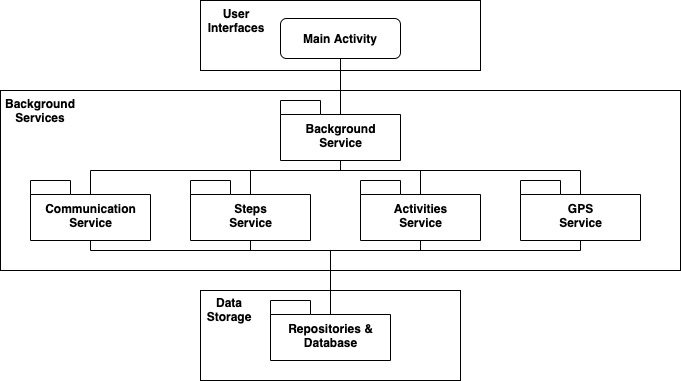
\includegraphics[width=0.8\textwidth]{figures/modules}
  \caption{Overview of the Android architecture} \label{fig:modules}
\end{figure}

On starting up, the application opens into the \textit{Main Activity}, where it asks the users for permission to access location services. On acceptance, the application starts the background services for data collection explained in the next section. It also serves the purpose of displaying stored data. A screen for each type is implemented: steps, activities, and GPS. Using Simon van Endern's Android application as a blueprint, we implement the same features to keep our application running behind the scenes. Because of background limitations Android introduced with Android Oreo, we create a non-dismissible notification that is displayed in the status bar and the notification center. This turns the application into a foreground application, bypassing the limitations set in the newer Android versions. To keep user interaction to a minimum, we enable the application to reopen when it crashes or is closed, and when it is rebooted.

\subsection{Data Collection}
After the users successfully accept all permissions, the \textit{Main Activity}, starts the \textit{Background Service}. The \textit{Background Service}, in turn, starts four tasks that have been shown in Figure \ref{fig:modules}. The four modules are loosely coupled and have been separated by data type or task at hand. We split the application into data collection and data aggregation. The aggregation process will be further explained in the next section. The data collection has three modules:
\begin{itemize}
    \item \textit{Steps Service}: This module handles two classes, the step service, and the step logger. If the mobile phone has a pedometer, it registers the sensor to update the step count. The step logger receives steps from the sensor and stores it in the \textit{steps\_table} ever minute. Every step entry has an \textit{start} and \textit{end} timestamp and the number of steps taken in that time frame as \textit{steps}.
    \item \textit{Activities Service}: This service, similar to the \textit{Steps Service}, is composed of the activities service and the activities logger classes. The activities service leverages Google's Activity Recognition API to identify the current activity of the mobile device. We are only interested in the main activities: still, walking, running, on a bicycle or in a vehicle. Therefore, for all possible activities, we register the transition type of entering or exiting the activity. Whenever we switch activities, the activities logger writes the \textit{timestamp}, the \textit{type} and wether we \textit{enter}ed or not into the \textit{activities\_table}. Additionally, we store the exited activity into the \textit{activitiesDetailed\_table} with the \textit{start} and \textit{end} timestamp and the \textit{type}.
% Todo: \cite[https://developers.google.com/android/reference/com/google/android/gms/location/DetectedActivity]
     \item \textit{GPS Service}: This part of the application has the same structure as the others described above. The GPS service accesses Google's Fused Location Provider API to collect location data. The API itself uses the GPS sensor as well as the network sensors in the device to determine device location. We make the location sample rate dependent on the current activity because the positional changes between \textit{still} and \textit{on a bicycle}, for example, are very different. So we set the interval to 5 minutes for \textit{still}, 30 seconds for \textit{walking} and 15, 5 and once per second for \textit{running}, \textit{on a bicycle} and \textit{in a vehicle} respectively. Every once in a while, the GPS logger receives batches of data from the API and saves them into the \textit{gps\_table} with their  \textit{timestamp}, \textit{lat}itude and \textit{lon}gtitude.
\end{itemize}

\subsection{Aggregation}
The last part of the background services is the \textit{Communication Service}. This is in charge of passing on data from the server or devices to the next target. For this interface, we have several ideas in mind.
 
\subsubsection{Peer-to-peer technology}
To take out the central server as an intermediary as implemented in Simon van Endern's version, we searched for libraries and SDKs that could be viable for our platform. We found the open-source projects, IPFS and libp2p, which are trying to be the foundation of the decentralized and distributed web. IPFS uses hashes to create content identifiers and turns them into blocks in a directed acyclic graph. To discover the peers with the content it uses a distributed hash table, using the modular P2P networking stack libp2p to communicate between nodes.
% Todo: \cite[IPFS] 

Textile leverages the strength of both technologies. Their main feature threads, a hash-chain of blocks that can represent any type of dataset, which we could use to send data directly from device to device. Unfortunately, after further investigation, the Textile SDK is not viable in its current state because it is unable to keep the node in Android alive after going into the background or turning off the device screen. It is essential for data collection and aggregation to keep communication channels available throughout the whole lifetime of the application.

Thus we opted to instead use a third-party push notification service as an intermediary to forward the messages between the server and other devices.

\subsubsection{Push}
To replace Simon van Ender's polling with an event-based action architecture, Figure \ref{fig:ar2} shows our new design. For our push service, we select Pushy
% Todo: \cite[Pushy]
because of their free entry barrier and independence from big tech companies, as well as having implementations for both iOS and Android. We could also have used Firebase Cloud Messaging to forward messages. Additionally, Pushy makes use of MQTT
% Todo: \cite[http://mqtt.org/]
, a light-weight messaging protocol that uses a small amount of bandwidth. Of course, the modular architecture of the app enables us to swap this method of communication for a P2P solution as soon as one proves applicable.

\begin{figure}[htbp]
  \centering
  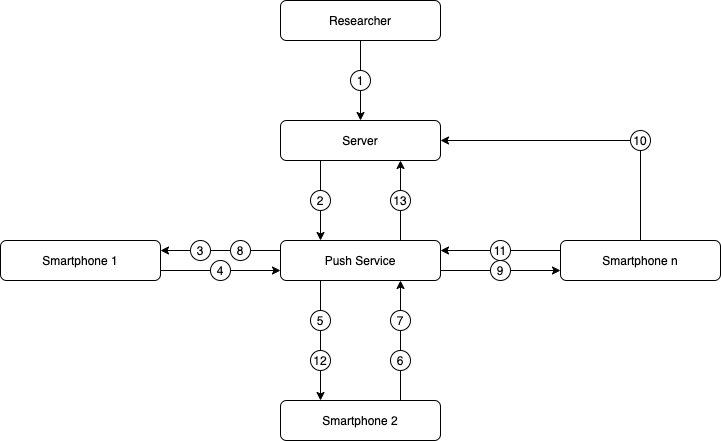
\includegraphics[width=0.8\textwidth]{figures/ar2}
  \caption{Data flow of an aggregation inside a group} \label{fig:ar2}
\end{figure}

\begin{enumerate}
	\item Researcher sends aggregation request to central server
	\item Server sends request push service
	\item Push service forwards request to first device
	\item Device adds data and sends results to push service targeting next device
	\item Push service forwards request to next device
	\item Device adds data and sends results to push service targeting next device
	\item Device sends confirmation message to push service targeting previous device
	\item Push service forwards confirmation to previous device
	\item Push service forwards request to next device and repeat until last device
	\item Last device adds data and sends results back to the server.
	\item Last device sends confirmation message to push service targeting previous device
	\item Push service forwards confirmation to previous device
\end{enumerate}

The complete communication infrastructure is handled by the communication service, communication receiver, and communication handler. After starting the application, the \textit{Background Service} creates the communication service that registers the device to the push service and receives a token as identification. Then it generates an asymmetric RSA key pair and registers itself to our platform with the Pushy token as \textit{id} and the \textit{publicKey} over the REST API. As a reply, the mobile phone receives a random password for future authentication purposes mentioned previously.

The communication receiver works as the entry point for push notifications from the push service and adds relevant data to the message. Upon receiving an aggregation request like in Listing \ref{lst:aggregation}, it checks for encryption and, if required, decrypts the data field. The application then aggregates data according to the \textit{type} sent in the \textit{requestHeader}:
\begin{itemize}
    \item \textbf{steps}: We add up the number of steps from the start and end of the specified day and add it to the list of raw values.
    \item \textbf{activities}: In this case, we sum up the time spent on the specified activity in the defined time frame and add that to the list of raw values.
    \item \textbf{location}: Here, we look for locations with the closest timestamp to the date specified in the header, but also inside a reasonable time, i.e., 10 minutes to cover the fact that still activities only logs the GPS data every 5 minutes. Then we spatially cloak the GPS coordinates and add it to the list of raw values as the hidden GPS position.
    \item \textbf{presence}: We just check all the GPS coordinates in the specified time frame, if they have been inside the range of the point of interest and add a 1 for if it has been and a 0 it has not.
\end{itemize}

After that, the communication handler takes the message and prepares it for the next participant in the \textit{group} array encoded in \textit{requestOptions}. If the device was the last in the list, it sends the results back to the server; otherwise, it uses the hybrid encryption scheme to encrypt data with the credentials of the subsequent device. So the current device generates a symmetric AES key and encrypts the \textit{data} and afterward does the same to the symmetric key using the public RSA key of the selected participant. Next, the communication handler forwards it over the push service, which in turn sends a push notification to the specified mobile phone. This repeats in each group until the last device has been chosen.

\subsubsection{Bypassing inactive users in the aggregation chain}
In the case, that the aggregation is stuck because of any reason, for instance, a device does not have an internet connection, it is turned off, or the participant deleted the application, we have to be able to bypass the inactive mobile phone and select a new one.

With our selected push notification service, the mobile phones periodically ping the push notification server, signaling that they are online and active. Using this information, we only send aggregation requests to the participants that are marked online by the service, bypassing devices that have been offline and have not contacted it in a while. But it could also be the case that the mobile phone is not available after the aggregation has already started.

So after the users forward their encrypted results to the following device, they start a sleeping thread that will skip the next device and select the one after that. The subsequent user that receives the message from the push service will aggregate the data as usual but will send a short confirmation message back to the preceding participant, which cancels the sleeping thread, signaling that aggregation was successful. The device does not need to be skipped.

By avoiding offline devices and actively confirming that a request has been fulfilled, we are able to bypass inactive users and make the aggregation more efficient and reliable.

\subsubsection{Spatial Cloaking}
To be able to provide k-anonymity for location data, we have to be able to generalize the GPS coordinates. By using spatial cloaking algorithms, we can hide the true position and hide the identifying landmarks by assigning the user to an approximate area. Normally, spatial cloaking algorithms try to minimize the area covered by spanning the cloaked region using the devices as corner points or border points. This, however, would reveal the actual locations of the participants if for k-anonymity k=2. So, we consider using Casper, Interval Cloaking, or Hilbert Cloaking. We select a variant of the Interval Cloaking algorithm by rounding down and rounding up the digit after the comma defined in \textit{accuracy} in the \textit{requestData} to create a rectangular area. To conserve data, we calculate the midpoint between the left lower corner and right upper corner of the area as a representative. It is important to find a good value for \textit{accuracy} because a high value results in a lot of suppression and a low value in generalized data. 

\subsubsection{Differential Privacy}
Differential privacy is a very powerful tool that can guarantee privacy. On the one hand, global differential privacy provides accurate data representation, but the algorithm needs the real values of the data infringing on our privacy-preserving requirement. Local differential privacy, on the other hand, can provide privacy without the intermediate data collector because of its composition feature. A disadvantage that local differential privacy brings is the necessity for a large data set. Since the noise addition to every entry in the set creates a much higher total noise level than global differential privacy and a huge number of participants is needed to cancel that out. 

Differential privacy heavily depends on the sensitivity of the data. That is the maximum value a single entry in the data set can change the query. For example, a query for the count of true and false answers; the sensitivity is one as the removal of one participant only removes one response of true or false. But the higher the sensitivity, the greater the noise that has to be added to the data to guarantee privacy, which in subsequently makes the data less accurate.

We considered implementing differential privacy, but ultimately decided against it. The global mechanism requires the server to have access to all raw values, while the local approach would add too much noise. In addition, differential private algorithms can currently only applied to simple data schemes, such as sums and counts, which would work with steps, activities and presence data, but couldn't be applied to location. Also, because of the high sensitivity of the values, because of our lack of participants, we are unable to cancel out the accumulated noise, basically making our collected data useless.

\section{Server}
For our server, we are using Node.js,
% Todo: \cite[https://nodejs.org/en/]
on version 12.12.21 with the express middleware, a minimal web application framework.
% Todo: \cite[https://expressjs.com/]
Our MongoDB Atlas database instance
% Todo: \cite[https://www.mongodb.com/cloud/atlas]
receives data over the database communication module. The architecture can be seen in Figure \ref{fig:server}.

\begin{figure}[htpb]
  \centering
  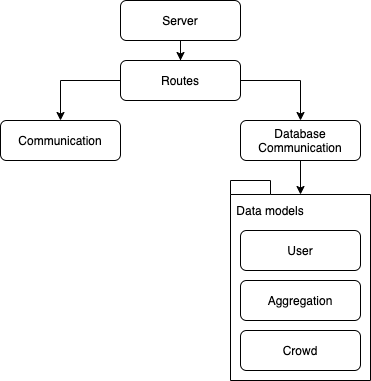
\includegraphics[width=0.5\textwidth]{figures/server}
  \caption{Overview of the server architecture} \label{fig:server}
\end{figure}

As our programming language, we select Typescript because of its versatility. As a superset of Javascript, it supports all Javascript libraries natively and allows for object-oriented programming paradigms. Also, it provides optional static typing and better code structure. But to run the server, we transpile our Typescript code to Javascript code to run the webserver.

When we start the server, \textit{app.ts} registers the routes described in the Table \ref{tab:rest} and connects the database object to the cloud storage instance. All calls to MongoDB are handled over that object, while the route handler manages calls to the endpoints.

\subsection{Registration}
Upon starting the application, it registers to the server using the JSON shown in Listing \ref{lst:registration} over the \textit{/crowd} route. To update the latest timestamp, we also have an obsolete route \textit{/crowd/ping}, which has been replaced with the ping our push notification service already provides. But this route can be modified to ping the devices for their current status if another communication model is adapted.

\subsection{Aggregation}
We create one route to which the researchers can send their aggregation requests. After receiving a JSON in the mentioned form in the Listing \ref{lst:request} in route \textit{/aggregationRequest}, the server will get all the devices, ping them using the push service, select all the available participants and calculate the groups. Before assigning the groups, we use the Fisher-Yates shuffle to mix the order of the users. We calculate group sizes depending on a designated minimal length, so the aggregation has enough members in each group for anonymity purposes, but small enough to stay efficient. After all that, the server sends the aggregation request to all groups using the push service.

On request creation, the server creates a temporary aggregation object that stores the id, number of groups, and how many it already has received. We have four additional routes for the final aggregation, \textit{/aggregationsteps}, \textit{/aggregationactivity}, \textit{/aggregationlocation} and \textit{/aggregationpresence}. They each manage the POST requests from the Android devices and calculate data or ensure anonymity.

\subsection{Anonymity}
To achieve privacy with data as sensitive as whereabouts, we apply k-anonymity. For steps and activity, we do not see any immediate privacy issues and thus refrain from using k-anonymity as that would needlessly sacrifice the usability of the data without benefits. As opposed to location data, we merge the received spatially cloaked raw values and suppress all coordinates that do not fulfill our defined k. 

\section{Limitations}
Even with the proposed solutions, the architecture is still far from perfect. While the data should be confidential because of the state-of-the-art encryption, we still have to rely on a third party to deliver messages, making us dependent on their availability.

With Simon van Endern's aggregation chain, the most vulnerable participants would be the first because next in line would always be able to see the raw data they added. Unfortunately, homomorphic encryption is still computationally expensive, and there are currently no available libraries for Android to implement it.

Another issue that can lead to privacy issues is centralization. While the raw data itself is distributed, the control over aggregated data, its storage, and its collection is still under one central authority.